\documentclass[a4paper]{article}
\usepackage[titletoc]{appendix}
\usepackage[a4paper,includeheadfoot,left=2.5cm,top=1.5cm,right=2.5cm,bottom=1.75cm]{geometry}
\usepackage{CJKutf8}
\usepackage{fancyhdr}

\usepackage{amsmath,amssymb,amsthm}
\usepackage{color,graphicx,subfigure,enumerate,epsfig,epstopdf}
\usepackage{pdfpages}

\title{Project Report for SMALLC}
\author{Li Wei (5092029004)}
\date{\today}

\begin{document}

\maketitle

\section{Introduction}

This project consist of 10 files described as follows.\\
\begin{enumerate}
  \item \texttt{smallc.l} is the lexical specification for \texttt{flex}.
  \item \texttt{smallc.y} is the syntactic specification for \texttt{bison}.
  \item \texttt{smallc.h} declares the data structure of \texttt{ast\_node, type\_node, scope\_node, sym\_node} and other functions prototypes which are used through out the building of the compiler.
  \item \texttt{main.c} contains the \texttt{main()} function which drives the whole parsing process.
  \item \texttt{ast.c} implements functions required for building the AST, type table, symbol table and scopes.
  \item \texttt{print\_ast.c} implements functions required for printing the AST in HTML format.
  \item \texttt{check\_ast.c} implements functions required for checking the AST types according to scopes.
  \item \texttt{generate\_ast.c} implements functions required for generating the MIPS code.
  \item \texttt{report.pdf} illustrates the design and implementations of the compiler
\end{enumerate}

\begin{figure}
  \centering
  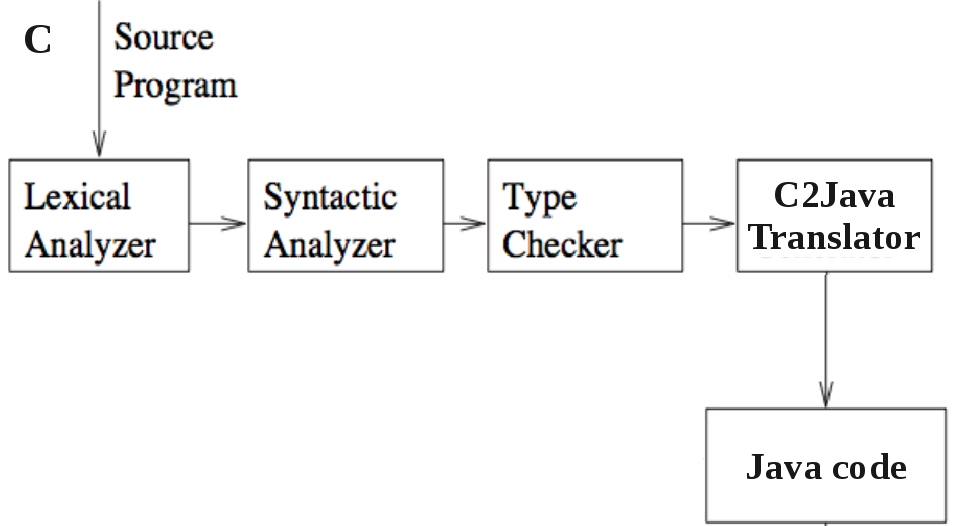
\includegraphics[width=0.9\textwidth]{overview}
  \caption{Compiler structure}
  \label{fig:overview}
\end{figure}


In my project, the stucture of the compiler is as shown in Figure \ref{fig:overview}. First the lexical analyzer takes the source program as input and output the tokens. Then the syntax analyzer will parse the tokens to construct the abstract syntax tree. Type checker will check the type rules of the abstact syntax tree. Finally the generator will generate MIPS code. Through this path, the ast\_node pass its five synthesized attributes: \texttt{int type\_id, int offset, int framesize, int lvalue, char fg};




\section{Lexical Analysis}

4 types of tokens are matched in the following order:
\begin{description}
  \item[Keywords:] \texttt{break}, \texttt{continue}, \texttt{if}, \texttt{else}, \texttt{for}, \texttt{int}, \texttt{return}, and \texttt{struct}, \texttt{read}.
  \item[Identifiers:] \texttt{sym()} function will look up the symbol table according to \texttt{yytext}.
  \item[Numbers:] hexadecimal, octal, and decimal integers.
  \item[Operators:] single-character operators correspond to the ASCII codes of the characters, while multiple-character operators have their own token numbers.
\end{description}
Whitespace and illegal characters are ignored. See \texttt{smallc.l} for details.



\section{Syntactic Analysis}

Non-terminals correspond to pointers of AST nodes with type \texttt{struct ast\_node}, which is defined in \texttt{smallc.h}.
For terminals, only \texttt{CONSTANT} and \texttt{IDENTIFIER} have values which are integers.
\texttt{CONSTANT} values are parsed integers. \texttt{IDENTIFIER} values are numeric symbols.\\

The grammar is a little different from that provided by the project description, e.g.\\
(i) avoiding sloppy $\epsilon$'s to reduce unnecessary conflicts;\\
(ii) using left recursions instead of right recursions to reduce backtracks and memory cost.\\
Also, operator precedence is implemented in a rather formal way other than specifying priorities to related tokens.\\


The abstract syntax tree will be constructed during the syntactic parsing by adding semantic actions. In the yacc program, the corresponding construct functions such as \texttt{funcdef\_new()} or \texttt{stdef\_new()} will be called at certain productions to construct the ast\_node of funcdef type or of stdef type.\\


The ast\_node defined in \texttt{smallc.h} has the different types, for instance \texttt{AST\_LIST, AST\_FUNCDEF, AST\_FUNCHEAD, AST\_PARA}. Each type has its own attributes implemented by a union. Details can be seen in \texttt{smallc.h}.\\


The construction functions are implemented with polymorphism, according to the type of the ast\_node, so as to in accord with the attributes of different types of ast\_node.

\section{Print Abstract Syntax Tree}


This part is for testing the constructed abstract syntax tree in the first part of the project. It isn't included in the final compiler as we only need to generate the MIPS code.

The ast will be printed by \texttt{print\_ast()}. For the sake of printing the parse tree in a hierarchical style, the list representation in HTML with tags $<ul>$ and $<li>$ is leveraged. Below is one instance for printing funcdef ast\_node.

\begin{verbatim}
static void print_funcdef(ast_node *n)
{
    printf("<ul>\n");
    printf("<li>funcdef</li>\n");
    printf("<li>ret_type: %d</li>\n", n->funcdef.ret_type);
    printf("<li>funchead:\n");
    print_ast(n->funcdef.funchead);
    printf("</li>\n");
    printf("<li>funcbody:\n");
    print_ast(n->funcdef.funcbody);
    printf("</li>\n");
    printf("</ul>\n");
}
\end{verbatim}

\begin{figure}
  \centering
  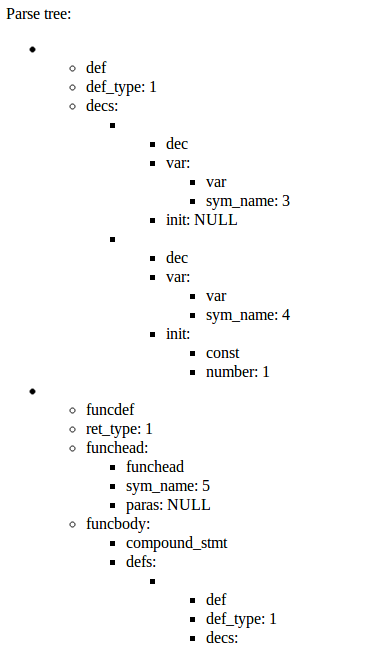
\includegraphics[width=0.5\textwidth]{printast}
  \caption{Print abstract syntax tree}
  \label{fig:printast}
\end{figure}


The parser reads from the input and writes the AST in HTML format to the output. 
It will create an HTML file to show the parse tree in a hierarchical way. One example is shown in Figure \ref{fig:printast}.


\section{Type Checking}

\begin{figure}
  \centering
  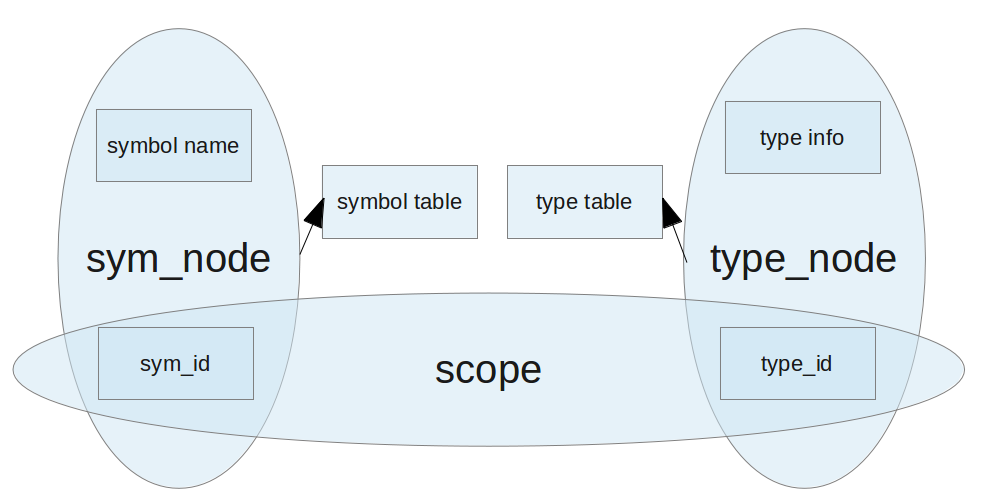
\includegraphics[width=\textwidth]{scope}
  \caption{Scope structure}
  \label{fig:scope}
\end{figure}

For type checking, I construct type table as well as the scopes. I seperate the scope into two scopes: vscope for variables and function names; tscope for new struct type names. The sym\_id and type\_id is stored in scope\_node. The type table contains the type infomation and the symbol talbe contains the hash from the string symbol name to int symbol id. The structure of the scope and the two tables are shown in Figure \ref{fig:scope}.\\

There are four types in my smallc: INT, STRUCTURE, ARRAY, FUNC. The information for each type is stored in type table, which is a list of type\_node. The data structure of type\_node is as below:

\begin{verbatim}
enum TYPE {STRUCTURE, ARRAY, FUNC};

struct field_list
{
	int sym_id;
	int index;
	struct field_list *next;
};

struct type_node
{
  int type_id;
  enum TYPE ty;
  union
  {
    struct
    {
      int sym_name;
      struct field_list *fields;
    } as_struct;
    
    struct 
    {
      int elem_type_id;
      int size;
    } as_array;
    
    struct
    {
      int ret_type;
      int para_num; 
      int para_type[1000];
    } as_func;
    
  };
  int mem_space;
  struct type_node *next;
};

\end{verbatim}
The type\_id for INT is always set to 1, so there's no need to store the INT type in the type table. The implementation here is the same with that in ast\_node, different attributes for different types in a union.\\


Here the array type contains three types: \textbf{INT, STRUCTURE and ARRAY}, which means it can have nesting arrays. So when constructing array in \texttt{check\_ast.c}, each nested array are given a type\_id by calling \texttt{array\_type()} to construct the array with setting up the attributes such as mem\_space in type\_node of array type.\\
The struct type only contains INT type.The function's return type and parameters' type can only be INT.
 

In my compiler, I implement the following type checks:
\begin{enumerate}
    \item Reserved words can not be used as \textit{identifiers}.
    \item Program must contain a function \textit{int main()} to be the entrance
    \item Check variables should not be re-declared by checking the curent scope
    \item Check variables have been declared before usage by checking all the \textbf{scopes}
    \item Check the initialized element have the same type with the left variable
    \item Check the size of the \textbf{array initialization} should equal or less than the size of the left array.
    \item Check the return type of function declaration should be INT
    \item Check function name should not be re-declared
    \item Check the parameter's type should be INT
    \item Check \textbf{parametes} should not have the same name
    \item Check if the structure type has been declared
    \item The condition of \textit{if} statement should be an expression with \textit{int} type
    \item Check wheather \textit{break} and \textit{continue} are in for loop
    \item The condition of \textit{for} should be an expression with \textit{int} type or epsilon
    \item Check the type of return statement in function should be INT
    \item Check only expression with type int can be involved in arithmetic
    \item Check right-value can not be assigned by any value or expression
    \item Use [] operator to a non-array variable is not allowed
    \item Check the \textit{identifier} of a function call is declared and is of type FUNC
    \item Check the number and type of variable(s) passed should match the definition of the function
    \item Check . operator can only be used to a struct variable
    \item Check the member following . operator is declared in the struct type
    \item Check the \textit{identifier} is declared
\end{enumerate}

Through type checking, the \texttt{check\_ast.c} also implements the following funtionalities:
\begin{itemize}
    \item Construct array type: array type can be constructed by STRUCT, INT and ARRAY type.
    \item Assign type id which is the synthesized attribute of the ast node
    \item Assign offset in the ast node of each declared variables
    \item Record whether the variable is left-value or right-value by assigning lvalue int each ast node to be 1 or 0
    \item Record the global variable and local variable in \texttt{char gf} in ast\_node
\end{itemize}


\section{Code Generation}

The implementation of the code generation part is similar with the checking and printing part. An array of function pointer will point to a specific function according to the type of the ast\_node. Below is the example of generate\_ast: 

\begin{verbatim}

static ast_generator g_ast_generators[AST_TYPE_LIMIT];

static void init_ast_generators()
{
    if (g_ast_generators[0]) return;

    g_ast_generators[AST_LIST] = gen_list;
    g_ast_generators[AST_FUNCDEF] = gen_funcdef;
    g_ast_generators[AST_FUNCHEAD] = gen_funchead;
    g_ast_generators[AST_PARA] = gen_para;
    g_ast_generators[AST_STDEF] = gen_stdef;
    g_ast_generators[AST_VAR] = gen_var;
    g_ast_generators[AST_SUBVAR] = gen_subvar;
    g_ast_generators[AST_COMPOUND_STMT] = gen_compound_stmt;
    g_ast_generators[AST_EXPR_STMT] = gen_expr_stmt;
    g_ast_generators[AST_IF_STMT] = gen_if_stmt;
    g_ast_generators[AST_FOR_STMT] = gen_for_stmt;
    g_ast_generators[AST_RETURN_STMT] = gen_return_stmt;
    g_ast_generators[AST_CONTINUE_STMT] = gen_continue_stmt;
    g_ast_generators[AST_BREAK_STMT] = gen_break_stmt;
    g_ast_generators[AST_DEF] = gen_def;
    g_ast_generators[AST_DEC] = gen_dec;
    g_ast_generators[AST_BINOP] = gen_binop;
    g_ast_generators[AST_PREFIX] = gen_prefix;
    g_ast_generators[AST_POSTFIX] = gen_postfix;
    g_ast_generators[AST_INDEXING] = gen_indexing;
    g_ast_generators[AST_FUNC_CALL] = gen_func_call;
    g_ast_generators[AST_MEMBER] = gen_member;
    g_ast_generators[AST_ID] = gen_id;
    g_ast_generators[AST_CONST] = gen_const;
}

\end{verbatim}

\begin{figure}
  \centering
  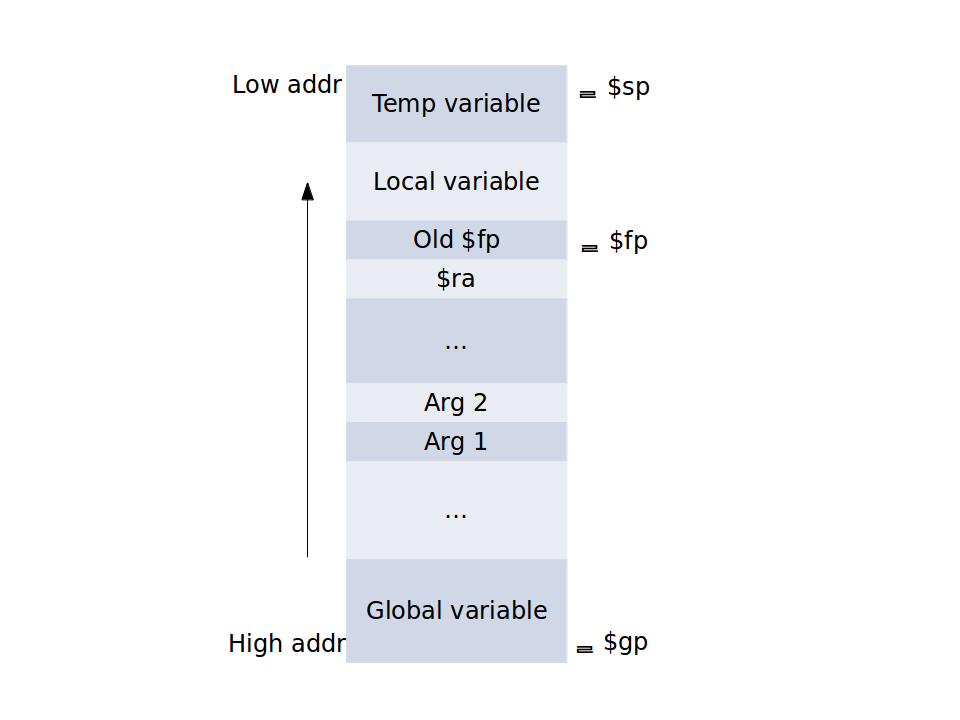
\includegraphics[width=0.7\textwidth]{smallc-stack}
  \caption{Stack}
  \label{fig:stack}
\end{figure}

The stack status in my implementation of smallc is shown in Figure \ref{fig:stack}.\\

The framesize of function is calculated in the type checking part and is used in function call part.\\
The offset of variable ast\_node is set when doing type checking and the temporary result will be stored in the new offset by calling \texttt{newtemp()}. There are some points we need to pay attention when implementing the generators:

\begin{itemize}
    \item The arguments of function should be put into stack in order. As the paramenters in fuction define is put into stack from high address to low address sequentially, the arguments should be in accord with the parameters. These can be done in setting the offset.
    \item The global data should be stored together. But they may not be written together in the source code. So a buffer is set to store all the global variables firest and settled them first before generating other mips code.
    \item Lazy evaluation is used when address the $\&\&$ and $||$ operators.
    \item In array initialization, each member in the initialization expression will be passed to be stored in the corresponsding offset of the members in array. If any members unassigned in the array, they will be set to 0.
    \item {\tt read(x)} is transformed to {\tt x = read()} in the parser in order to be processed consistently along with other function calls.
    \item Both {\tt read} and {\tt write} are considered as standard library functions, and implemented in MIPS as follows.
\begin{verbatim}
.data 
.align 2
newline: .asciiz "\n"
.text
.align 2
read_1:
  li $v0, 5             # read_int
  syscall
  jr $ra
write_2:
  lw $a0, ($sp)
  li $v0, 1             # print_int
  syscall
  la $a0, newline
  li $v0, 4             # print_string
  syscall
  jr $ra
\end{verbatim}
    \item {\tt void gen\_lvalue(ast\_node *n)} saves the address of the {\tt ast\_node} in {\tt \$t9} in order to be used as the lvalue.
\end{itemize}

\end{document}
